\chapter{Adaptierbarkeit}
\label{ch:adaptierbarkeit}
Die in Kapitel~\ref{ch:neuronalesNetz} auf Seite~\pageref{ch:neuronalesNetz} aufgebaute und erstellte Architektur soll
zusammen mit dem in Kapitel~\ref{ch:client} auf Seite~\pageref{ch:client} implementierten Frontend durch weitere Ideen
erweitert und verbessert werden.

Eine Untersuchung soll ergeben, ob sowohl die Architektur als auch das Frontend so modular entwickelt wurden, dass sie 
problemlos durch weitere Funktionen und Ideen erweitert werden können. Eventuell Probleme im System sollen gelößt werden.

Dies ist zwingend erforderlich um zum Beispiel eine weitere Maschinen oder neue Module ebenfalls in das System zu 
integrieren, um auf neue Versionen oder neu herausgebrachte Maschinen reagieren zu können.

Für dieses Ziel werden in den folgenden Kapitel mehrere Ideen für passende Erweiterungen behandelt und diese Schritt für 
Schritt umgesetzt und eingebaut.

Die Abbildung~\ref{fig:schematische_architektur_5} auf Seite~\pageref{fig:schematische_architektur_5} zeigt eine schematische 
Erweiterung des Systems. Dort ist sehr gut ersichtlich, dass der API Connect eine zentrale Rolle in der Erweiterbarkeit 
einnimmt.

\begin{figure}[h]
    \centering
    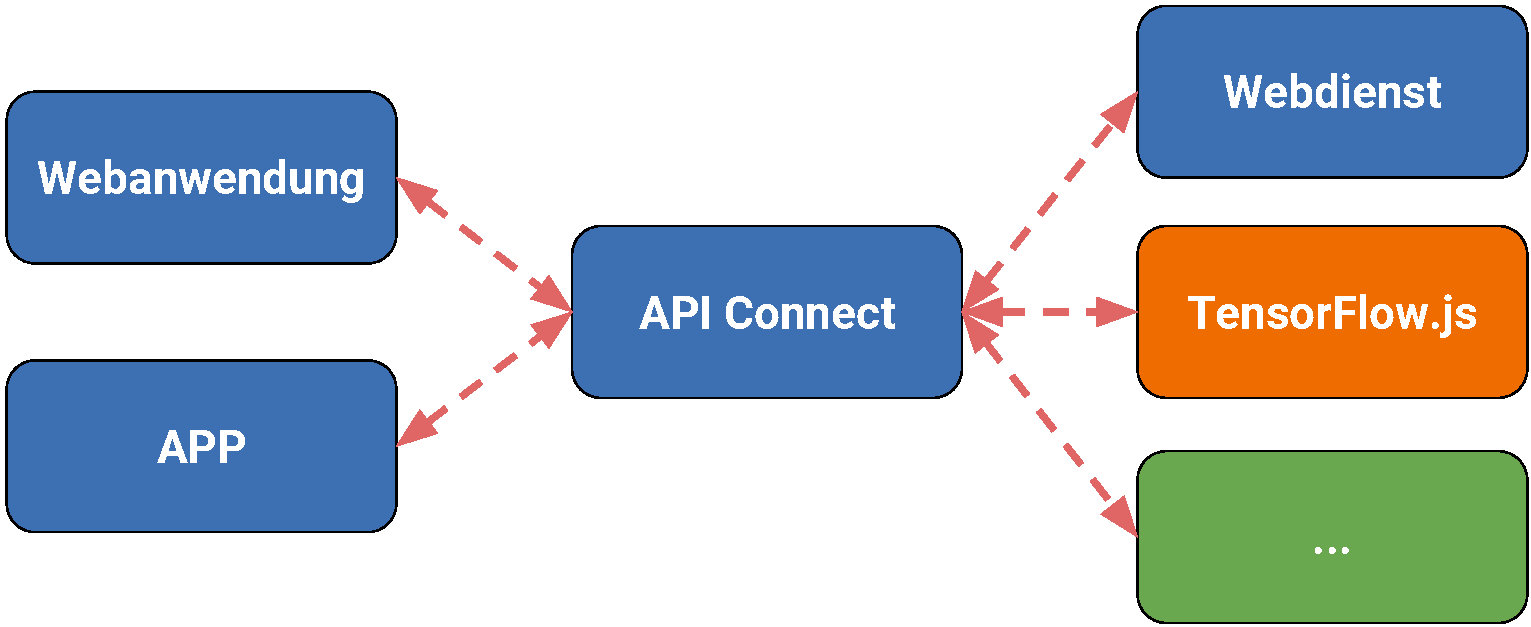
\includegraphics[width=\textwidth]{images/kapitel_5/architektur_schematisch.pdf}
    \caption{Schematische Darstellung der Architektur}
    \label{fig:schematische_architektur_5}
\end{figure}